%\documentclass[landscape,a0b,a4resizeable,draft]{a0poster}
\documentclass[landscape,a0b,final]{a0poster}

%%% Option "a4resizeable" makes it possible ot resize the
%   poster by the command: psresize -pa4 poster.ps poster-a4.ps
%   For final printing, please remove option "a4resizeable" !!

%Compile at the command prompt via
%dvips -Ppdf poster.dvi -o poster.ps
% then
% ps2pdf poster.ps poster.pdf

\usepackage{enumerate}
\usepackage{epsfig}
\usepackage{multicol}
\usepackage{amsmath}
\usepackage{amssymb}
\usepackage{psfrag}
\usepackage{pstricks,pst-grad}


%%%%%%%%%%%%%%%%%%%%%%%%%%%%%%%%%%%%%%%%%%%
% Import Header
\input defs.tex



%%%%%%%%%%%%%%%%%%%%%%%%%%%%%%%%%%%%%%%%%%%
% Definition of some variables and colors
%\renewcommand{\rho}{\varrho}
%\renewcommand{\phi}{\varphi}
\setlength{\columnsep}{3cm}
\setlength{\columnseprule}{2mm}
\setlength{\parindent}{0.0cm}
\newcommand{\norm}[1]{\left\Vert#1\right\Vert}
\newcommand{\abs}[1]{\left\vert#1\right\vert}
\newcommand{\nn}{\nonumber}



%%%%%%%%%%%%%%%%%%%%%%%%%%%%%%%%%%%%%%%%%%%%%%%%%%%%
%%%               Background                     %%%
%%%%%%%%%%%%%%%%%%%%%%%%%%%%%%%%%%%%%%%%%%%%%%%%%%%%

\newcommand{\background}[3]{
  \newrgbcolor{cgradbegin}{#1}
  \newrgbcolor{cgradend}{#2}
  \psframe[fillstyle=gradient,gradend=cgradend,
  gradbegin=cgradbegin,gradmidpoint=#3](0.,0.)(1.\textwidth,-1.\textheight)
}



%%%%%%%%%%%%%%%%%%%%%%%%%%%%%%%%%%%%%%%%%%%%%%%%%%%%
%%%                Poster                        %%%
%%%%%%%%%%%%%%%%%%%%%%%%%%%%%%%%%%%%%%%%%%%%%%%%%%%%

\newenvironment{poster}{
  \begin{center}
  \begin{minipage}[c]{0.98\textwidth}
}{
  \end{minipage}
  \end{center}
}



%%%%%%%%%%%%%%%%%%%%%%%%%%%%%%%%%%%%%%%%%%%%%%%%%%%%
%%%                pcolumn                       %%%
%%%%%%%%%%%%%%%%%%%%%%%%%%%%%%%%%%%%%%%%%%%%%%%%%%%%

\newenvironment{pcolumn}[1]{
  \begin{minipage}{#1\textwidth}
  \begin{center}
}{
  \end{center}
  \end{minipage}
}



%%%%%%%%%%%%%%%%%%%%%%%%%%%%%%%%%%%%%%%%%%%%%%%%%%%%
%%%                pbox                          %%%
%%%%%%%%%%%%%%%%%%%%%%%%%%%%%%%%%%%%%%%%%%%%%%%%%%%%

\newrgbcolor{lcolor}{0. 0. 0.80}
\newrgbcolor{gcolor1}{1. 1. 1.}
\newrgbcolor{gcolor2}{.80 .80 1.}

\newcommand{\pbox}[4]{
\psshadowbox[#3]{
\begin{minipage}[t][#2][t]{#1}
#4
\end{minipage}
}}



%%%%%%%%%%%%%%%%%%%%%%%%%%%%%%%%%%%%%%%%%%%%%%%%%%%%
%%%                myfig                         %%%
%%%%%%%%%%%%%%%%%%%%%%%%%%%%%%%%%%%%%%%%%%%%%%%%%%%%
% \myfig - replacement for \figure
% necessary, since in multicol-environment
% \figure won't work

\newcommand{\myfig}[3][0]{
\begin{center}
  \vspace{1.5cm}
  \includegraphics[width=#3\hsize,height=#1\vsize]{#2}
  \nobreak
\end{center}}

%%%%%%%%%%%%%%%%%%%%%%%%%%%%%%%%%%%%%%%%%%%%%%%%%%%%
%%%                mycaption                     %%%
%%%%%%%%%%%%%%%%%%%%%%%%%%%%%%%%%%%%%%%%%%%%%%%%%%%%
% \mycaption - replacement for \caption
% necessary, since in multicol-environment \figure and
% therefore \caption won't work

%\newcounter{figure}
\setcounter{figure}{1}
\newcommand{\mycaption}[1]{
  \vspace{0.5cm}
  \begin{center}
  \begin{quote}
    {{\sc Figure} \arabic{figure}: #1}
  \end{quote}
  \end{center}
  %\vspace{1cm}
  \stepcounter{figure}
}

%\defeq
%%%%%%%%%%%%%%%%%%%%%%%%%%%%%%%%%%%%%%%%%%%%%%%%%%%%%%%%%%%%%%%%%%%%%%
\newcommand{\defeq}{:=}
\newcommand{\fdiv}[2]{D_f\left({#1} |\!| {#2} \right)}
\newcommand{\mc}[1]{\mathcal{#1}}
%%%%%%%%%%%%%%%%%%%%%%%%%%%%%%%%%%%%%%%%%%%%%%%%%%%%%%%%%%%%%%%%%%%%%%

%%%%%%%%%%%%%%%%%%%%%%%%%%%%%%%%%%%%%%%%%%%%%%%%%%%%%%%%%%%%%%%%%%%%%%
%%% Begin of Document
%%%%%%%%%%%%%%%%%%%%%%%%%%%%%%%%%%%%%%%%%%%%%%%%%%%%%%%%%%%%%%%%%%%%%%

\begin{document}


\background{1. 1. 1.}{1. 1. 1.}{0.5}

\vspace*{2cm}


\newrgbcolor{lightred}{0.80 0. 0}
\newrgbcolor{white}{1. 1. 1.}
\newrgbcolor{whitered}{1. .80 .80}


\begin{poster}

%%%%%%%%%%%%%%%%%%%%%
%%% Header
%%%%%%%%%%%%%%%%%%%%%
\begin{center}
\begin{pcolumn}{0.98}

\pbox{0.95\textwidth}{}{linewidth=2mm,framearc=0.3,linecolor=lightred,fillstyle=gradient,
gradangle=0,gradbegin=white,gradend=whitered,gradmidpoint=1.0,framesep=1em}{

%%% Unisiegel
\begin{minipage}[c][9cm][c]{0.1\textwidth}
  \begin{center}
    
\includegraphics[width=7cm,angle=0]{figures/stanfordlogo.eps}
  \end{center}
\end{minipage}
%%% Titel
\begin{minipage}[c][9cm][c]{0.78\textwidth}
  \begin{center}
    {\sc \Huge Minimax Estimation of Simultaneously Low Rank and Sparse Matrices}\\[10mm]
    {\Large Yuanyuan Shen$^{1}$, Zi Yin$^2$ and Feng Ruan$^3$  \\[7.5mm]
    $^{1,3}$ Department of Statistics and $^2$ Department of Electrical Engineering, Stanford University}
  \end{center}
\end{minipage}
%%% GK-Logo
\begin{minipage}[c][9cm][c]{0.1\textwidth}
  \begin{center}
    
\includegraphics[width=7cm,angle=0]{figures/stanfordlogo.eps}
  \end{center}
\end{minipage}

}
\end{pcolumn}
\end{center}


\vspace*{1.5cm}
\newcommand{\R}{\textbf{R}}
\newcommand{\N}{\mathcal{N}}

%%%%%%%%%%%%%%%%%%%%%
%%% Content
%%%%%%%%%%%%%%%%%%%%%
\begin{center}
\begin{pcolumn}{0.30}
\pbox{0.9\textwidth}{65cm}{linewidth=2mm,framearc=0.1,linecolor=lightred,
fillstyle=gradient,gradangle=0,gradbegin=white,gradend=white,gradmidpoint=1.0,framesep=1em}{
%----------------------------------
%%% Introduction
%-----------------------------------
\vspace{0.5cm}
\begin{center}\pbox{0.8\textwidth}{}{linewidth=2mm,framearc=0.1,linecolor=lightred,
fillstyle=gradient,gradangle=0,gradbegin=white,gradend=whitered,gradmidpoint=1.0,framesep=1em}
{\begin{center}Introduction\end{center}}\end{center} \vspace{1cm}
%In recent years, there has been a surge of interest in estimating and denoising structured large matrices. 
In this project, we study the problem of estimating matrices with a simultaneous structure: \emph{low rank and 
sparsity}, under gaussian sequence and regression models. In both models, we use $\Theta^* \in \R^{p\times p}$ 
to denote the underlying sparse and low rank matrix. In gaussian sequence model, we observe some noisy matrix 
denoted by $X\in \R^{p\times p}$:
\begin{equation*}
\textbf{Gaussian Sequence Model} ~~~ X = \Theta^* + E~~~ E_{ij}\sim \N(0, \sigma^2),
\end{equation*}
while in the regression model, we observe the responses $y_i \in \R$ 
for $i=1,2, \ldots, N$ along with their covariates $x_i \in \R^p$:
\begin{equation*}
\textbf{Regression Model} ~~~ y_i = x_i^T \Theta^* x_i + \epsilon_i, \epsilon_i\sim \N(0, \sigma^2)
\end{equation*}
Our aim is to analyze the fundamental limits of estimation of such low-rank and sparse matrix
under the above models, using techniques borrowed from theoretical computer science and information theory. 

\vspace{0.2cm}
The two models can have many potential applications. For example, in genetic studies, biologists are interested in understanding the interactions 
between genes, where they often model the underlying interaction matrices to have certain bi-clustering structure.  
Such bicluster structure can be well-captured by simultaneous low-rank and sparse matrices if additional 
sparsity assumptions on groups of interactive genes are enforced. Similarly, in social network studies, 
a problem of major interest is the `community detection' problem, where sociologists need to construct the 
underlying adjacent matrix determined by hidden communities. One can characterize such matrices as 
simultaneously low rank and sparse matrices, as long as there are only a few different communities. 

\vspace{0.5cm}


%----------------------------------
%%% L1-norm ranking
%----------------------------------
\vspace{1cm}
\begin{center}\pbox{0.8\textwidth}{}{linewidth=2mm,framearc=0.1,linecolor=lightred,
fillstyle=gradient,gradangle=0,gradbegin=white,gradend=whitered,gradmidpoint=1.0,framesep=1em}
{\begin{center}Background and Related Work\end{center}}\end{center}
\vspace{0.5cm}
Here, we formalize the concept of low rank and sparse matrix. 
A matrix $A \in \R^{p\times p}$ is called simultaneously low-rank and sparse with parameters $(s, r)$ 
if there exist $u_i \in \R^p$ and $v_i\in \R^p$ with $\|u_i\|_0 \leq s$, $\|v_i\|_0 \leq s$, $\|u_i\|_2 = \|v_i\|_2 =1$,
and $\theta_i \in \R$ such that 
\begin{equation*}
A = \sum_{i=1}^r \theta_i u_i v_i^T.
\end{equation*}
In this project, our main focus is to evaluate the minimax rate of the estimation of 
sparse low-rank matrices with parameters $(r, s) = (1, s)$, i.e., all rank-one 
matrices that have only one $s$ by $s$ block. 
Note that, although our definition of simultaneously sparse and low-rank matrices 
is close to that appeared in [1], the resulting minimax rate for these two classes 
of matrices are in fact different, as [1] requires additional assumptions on 
top eigenvalues. In addition, the techniques that evaluate the 
minimax rate in our class of matrices are also fundamentally different 
from those appeared in [1]. 

To evaluate the minimax rate of estimation for our defined matrix class, we 
borrow ideas from literatures that focus on sparse PCA, e.g., [2], [3] and [4]. In 
these papers, the authors analyze the fundamental limits under some different yet 
similar models, where they need to estimate the top sparse eigenvector of some 
low rank and sparse covariance matrices.  
In their papers, the authors prove that, the $\ell_2$ minimax rate for estimation of 
the top eigenvectors is $\sqrt{s\log p/N}$ up to a constant. In addition to that, [4] shows
that roughly no convex procedures can actually achieve this minimax rate, and the price 
for convex procedures to pay is that a factor of $\sqrt{s}$ will appear in their $\ell_2$ error rate. 
In this project, we show that parallel results hold in the estimation of the entire matrices,
where both the top eigenvectors and corresponding eigenvalues are simultaneously estimated. 
The minimax $\ell_2$ rate for matrix estimation for the classes of matrices with $(r, s) = (1, s)$, 
to our surprise, is still $\sqrt{s\log p/N}$. 
We also provide a fast convex regularization procedure that can actually achieve the 
minimax $\ell_2$ rate within a multiplication factor of $\sqrt{s}$. This suggests that 
a deeper connection may exist between our estimation problem and sparse PCA problem.


\vspace{0.5cm}
}
\end{pcolumn}
\begin{pcolumn}{0.30}

\pbox{0.9\textwidth}{65cm}{linewidth=2mm,framearc=0.1,linecolor=lightred,fillstyle=gradient,
gradangle=0,gradbegin=white,gradend=white,gradmidpoint=1.0,framesep=1em}{
%----------------------------------
%%% Theory
%----------------------------------
\vspace{.5cm}
\begin{center}\pbox{0.8\textwidth}{}{linewidth=2mm,framearc=0.1,linecolor=lightred,fillstyle=gradient,
gradangle=0,gradbegin=white,gradend=whitered,gradmidpoint=1.0,framesep=1em}{\begin{center}
Main Results
\end{center}}\end{center}
\vspace{1.25cm}

\psshadowbox[linewidth=1mm,framearc=0.1,linecolor=red,framesep=1em]{
\begin{minipage}[h]{0.94\linewidth}
{\bf Proposition 1 [Minimax Rate for Gaussian Sequence Model]}\\
Under Gaussian sequence model, the minimax rate of the estimation of simultaneously low
rank and sparse matrix with parameters $(r, s) = (1, s)$ is $\asymp \sigma\sqrt{ s \log p}$. 
More precisely, there exist some universal constants $c, C, c_1, c_2 > 0$ such that 
\begin{equation*}
\inf_{\hat{\Theta}}\sup_{\Theta \in \Theta(1, s)} 
P \left( \|\hat{\Theta} - \Theta\|_F \geq c \sigma \left( \sqrt{s \log\frac{ p}{s}}   \right)\right) \geq \frac{1}{2}
\end{equation*}
\begin{eqnarray*}
\inf_{\hat{\Theta}}\sup_{\Theta \in \Theta(1, s)} 
P \left( \|\hat{\Theta} - \Theta\|_F \geq C \sigma\left( \sqrt{s \log \frac{p}{s}}   \right) \right) 
\leq  c_1\exp(-c_2 (s\log p/s )/\sigma^2), \\
\end{eqnarray*}
where 
\begin{equation*}
\Theta(r, s) = \left\{\Theta \in \R^{p\times p} \mid \Theta = \sum_{i=1}^r \theta_i u_i v_i^T, 
\|u_i\|_2 = \|v_i\|_2 = 1, \|u_i\|_0 \leq s, \|v_i\|_0 \leq s \right\}
\end{equation*}
 \end{minipage}
}

\vspace{0.7cm}

{\bf Remark 1}
Proposition 1 parallels the result in sparse PCA literature [3], where estimation of sparse eigenvector
achieves the same minimax error rate. (Note that $\sigma \asymp \frac{1}{\sqrt{N}}$).\\
{\bf Remark 2} 
The result can be generalized to the estimation problem of sparse and low rank rectangular matrix
with different height and width. 

\vspace{0.7cm}

\psshadowbox[linewidth=1mm,framearc=0.1,linecolor=red,framesep=1em]{
\begin{minipage}[h]{0.94\linewidth}
{\bf Proposition 2 [Soft-Thresholding achieves Sub-optimal Rate]}\\
Let $l_\lambda(x) \defeq \sign(x)(|x|-\lambda)_+$. Consider the following thresholding estimator $\hat{\Theta} \defeq
l_\lambda(X)$, where we do entry-wise soft thresholding on the observed matrix $X$. Then, if we choose 
$\lambda$ to be greater than $\sigma \sqrt{2\log p}$, then there exists some universal constants $c, C > 0$ such that 
\begin{equation*}
\|\hat{\Theta} - \Theta^*\|_F \leq C s \lambda
\end{equation*}
holds with probability greater than $1-p^{-c}$. 

\end{minipage}
}
\vspace{0.5cm}

{\bf Remark 3} 
Soft-thresholding is easy to compute in practice, yet the price to pay for the speed 
is the scaling of the statistical convergence rate by a factor of $\sqrt{s}$. 

\vspace{0.7cm}


\psshadowbox[linewidth=1mm,framearc=0.1,linecolor=red,framesep=1em]{
\begin{minipage}[h]{0.94\linewidth}
{\bf Proposition 3 [Minimax Rate for Regression Model]} \\
Assume the following regularity condition on the design matrix $X$: 
$\exists \kappa, \eta > 0$ such that $\forall \Delta \in \left\{ \Delta \mid \|\Delta\|_F = 1, \rank{\Delta} = 2\right\}$: 
\begin{equation}
\label{eqn: assumption}
\kappa \leq \frac{1}{N} \sum_{i=1}^N \left(x_i^T \Delta x_i \right)^2 \leq \eta.
\end{equation}
Then, the minimax rate of estimation of $\Theta^* \in \Theta(1, s)$ is $\asymp \sigma\sqrt{s\log p/s}$. 
More precisely, there exist some constants $c, C > 0$ and $c_1, c_2 > 0$ that are only dependent on 
$\kappa$ and $\eta$,  such that 
\begin{equation*}
\inf_{\hat{\Theta}}\sup_{\Theta \in \Theta(1,s)} 
P \left( \|\hat{\Theta} - \Theta\|_F \geq c \left( \sigma\sqrt{s \log \frac{ p}{s}} \right) \right) \geq \frac{1}{2}
\end{equation*}
\begin{equation*}
\inf_{\hat{\Theta}}\sup_{\Theta \in \Theta(1,s)} 
P \left( \|\hat{\Theta} - \Theta\|_F \geq C \left( \sigma\sqrt{s \log \frac{ p}{s}} \right) \right) 
\leq c_1\exp(-c_2 N(s\log p/s) )
\end{equation*}
\end{minipage}
}


\vspace{0.5cm}

}
\end{pcolumn}
\begin{pcolumn}{0.30}
\pbox{0.9\textwidth}{65cm}{linewidth=2mm,framearc=0.1,linecolor=lightred,fillstyle=gradient,
gradangle=0,gradbegin=white,gradend=white,gradmidpoint=1.0,framesep=1em}{


%----------------------------------
%%% Experiments
%----------------------------------
\vspace{1.0 cm}
\psshadowbox[linewidth=1mm,framearc=0.1,linecolor=red,framesep=1em]{
\begin{minipage}[h]{0.94\linewidth}
{\bf Proposition 4 [$\ell_1$ regularization achieves Sub-optimal Rate]}\\
Consider the following penalized $\ell_1$ regression: 
\begin{equation*}
\hat{\Theta} \defeq \argmin_{\Theta}  \frac{1}{N} \sum_{i=1}^N (y_i - x_i^T \Theta x_i)^2 + \lambda \|\Theta\|_1
\end{equation*}
Suppose assumption~(Eq.\ref{eqn: assumption}) on $X$ still holds. 
Then for any $\lambda$ that is greater than $2\sigma\sqrt{\log p/N}$, 
there exists some constants $c, C > 0$ that are only dependent on $\kappa$ and $\eta$ 
such that 
\begin{equation*}
\|\hat{\Theta} - \Theta^*\|_F \leq C s\lambda
\end{equation*}
holds with probably at least $1-p^{-c}$ 
\end{minipage}
}

\vspace{0.5cm}

{\bf Remark 4}
The assumption~Eq.\ref{eqn: assumption} can hold w.h.p in general random design as long as
the row of $X$ are i.i.d sampled from some distribution with compact support and the sample 
size $N = \Omega\left(\max\{s^3, s\log p\}\right)$

\vspace{0.5cm}
\vspace{1cm}
\begin{center}\pbox{0.8\textwidth}{}{linewidth=2mm,framearc=0.1,linecolor=lightred,
fillstyle=gradient,gradangle=0,gradbegin=white,gradend=whitered,gradmidpoint=1.0,framesep=1em}
{\begin{center}Simulation Studies\end{center}}\end{center} \vspace{1cm}
In our simulation setting, $p = 50$, $N = 100$, $r = 2$, $s = 3$. $\theta_1 = \theta_2 = 1$. 
The SPCA achieves better performance in both estimation and support recovery than that of 
the oracle lasso procedure. 

\begin{minipage}[c][\linewidth][c]{\linewidth}
  \begin{center}
    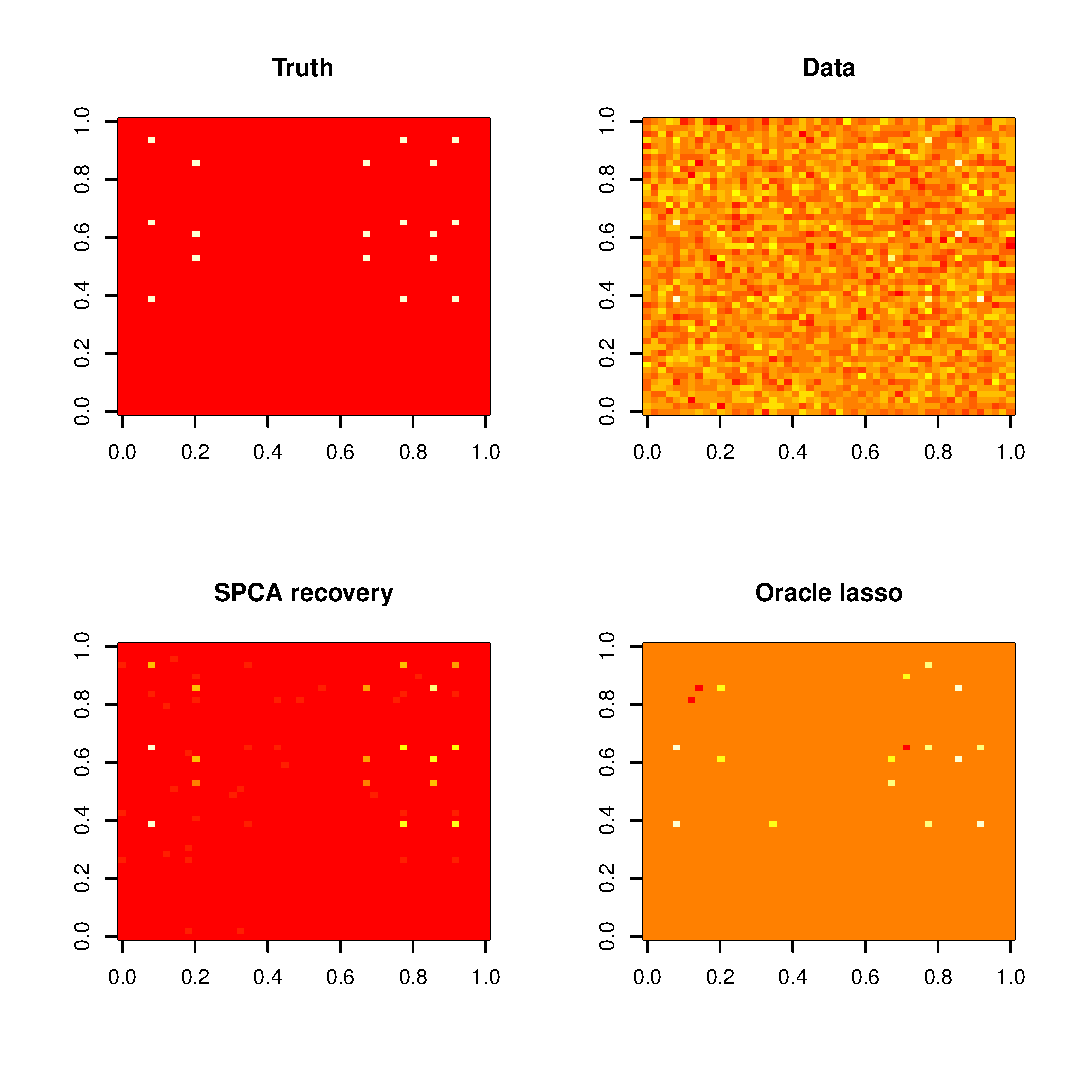
\includegraphics[width=\linewidth,angle=0]{figures/image.eps}
  \end{center}
\end{minipage}
\vspace{-2cm}
\begin{thebibliography}{5}
\bibitem{YZA14} D. Yang, Z. Ma and A. Buja. \emph{Journal of Machine Learning Research},  to appear.
\bibitem{AW09} A. Amina and M. Wainwright. \emph{The Annals of Statistics}, 2009, 37(5B): 2877-2921.
\bibitem{JL12} I. Johnstone and A. Lu. \emph{Journal of the American Statistical Association}, 2012. 
\bibitem{BP13} Q. Berthet and P. Rigollet. \emph{The Annals of Statistics}, 2013, 41(4):1780-1815.
\end{thebibliography}
}
\end{pcolumn}
\end{center}
\end{poster}
\end{document}
